\section{Componentes da DSL Cotas no \gls{MPS}}
\label{sec:mps}

Nessa Seção são descritos os elementos de modelagem criados na ferramenta \gls{MPS} tais como: os componentes de estrutura (\texttt{structure concepts}), a sintaxe dos editores projecionais (\texttt{editors}), restrições de escopo (\texttt{constraints}), comportamentos de conceitos (\texttt{behaviors}), sistema de tipos (\texttt{typesystem}) e, por fim, os elementos de geração de texto (\texttt{textGen}).

\subsection{\textit{Componentes de estrutura}}
\label{sub:sec:estrutura}

\textit{Concepts} ou conceitos no \gls{MPS} servem para definir a estrutura base da linguagem, cada conceito pode conter propriedades, outros conceitos filhos \texttt{childrens} e referências para outros conceitos. Eles podem herdar ou implementar características de outros conceitos. A Figura \ref{fig:structure} apresenta a lista de conceitos criados para a DSL Cotas.

\begin{figure}[ht!]
\centering

\caption{\textmd{Lista de Conceitos de Estrutura \gls{MPS}}}
\label{fig:structure}
\fcolorbox{gray}{white}{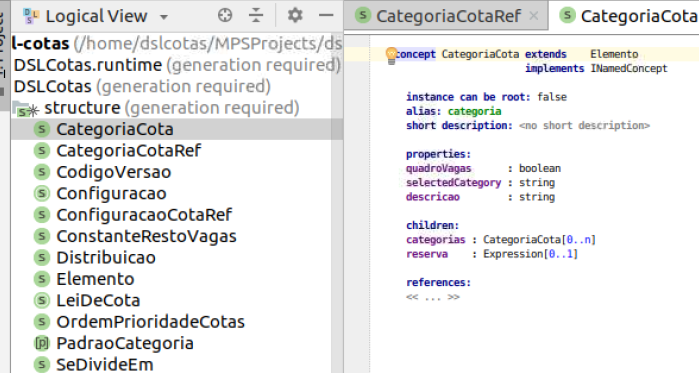
\includegraphics[width=0.70\textwidth]{chapters/dslcotas/mps/imagens/structure.png}}

\par\medskip\textbf{Fonte:} Elaboração do autor (2020) \par\medskip

\end{figure}





Esses conceitos definem a estrutura hierárquica da \gls{AST} de modo análogo ao modelo orientado a objetos, portanto, a Figura \ref{fig:classesmps} mostra a representação da modelagem dos conceitos em formato de diagrama de classes da \gls{UML}.

\begin{figure}[ht!]
\centering

\caption{\textmd{Modelo de Conceitos no \gls{MPS}}}
\label{fig:classesmps}
\fcolorbox{gray}{white}{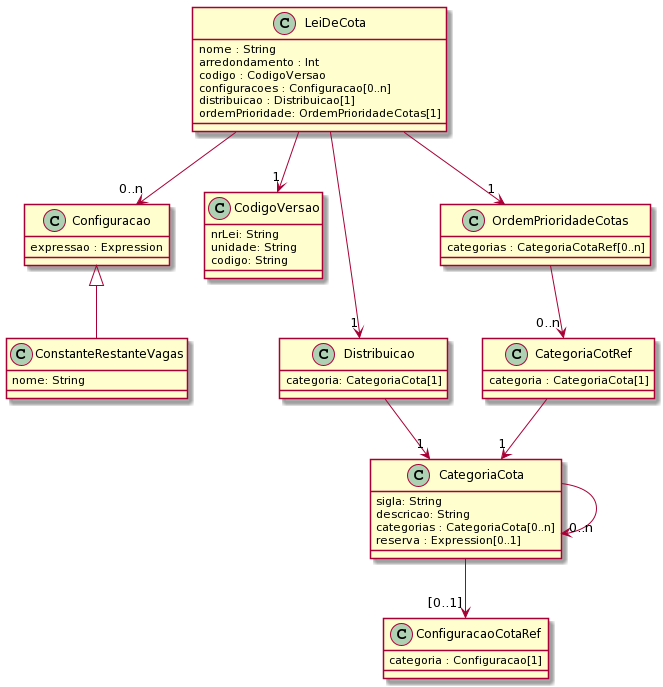
\includegraphics[width=0.70\textwidth]{chapters/dslcotas/mps/imagens/classesmps.png}}

\par\medskip\textbf{Fonte:} Elaborada pelo autor (2020). \par\medskip

\end{figure}




\newpage
O conceito \texttt{LeiDeCota} é o elemento raiz  que pode ser instanciado no \gls{MPS} a fim de criar uma representação abstrata de uma nova lei de cotas na DSL. No \gls{MPS}, os conceitos raiz podem ser criados em módulos \texttt{Solutions}, os quais utilizam uma ou mais linguagens e são os responsáveis por conter o código fonte do usuário final (Figura \ref{fig:solutions}).

\begin{figure}[ht!]
\centering

\caption{\textmd{Criação de elementos raiz em  \texttt{Solutions} no \gls{MPS}}}
\label{fig:solutions}
\fcolorbox{gray}{white}{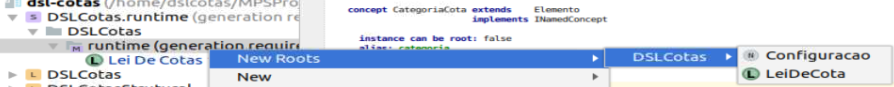
\includegraphics[width=\textwidth]{chapters/dslcotas/mps/imagens/solutions.png}}

\par\medskip\textbf{Fonte:} Elaboração do autor (2020) \par\medskip

\end{figure}



Por sua vez, uma \texttt{LeiDeCota} está associada aos elementos descritos na Tabela \ref{tblelementoslei}:

\begin{table}[ht]
\caption{Elementos associados ao conceito \texttt{LeiDeCota}}
\label{tblelementoslei}
\centering
\begin{tabular}{|p{4.2cm}|p{10cm}|}
\hline
\texttt{CodigoVersao}          & Elemento que mantém informações descritivas sobre a versão de lei aplicada.                                                                                           \\ \hline
Lista de \texttt{Configuracao} & Responsável por armazenar os parâmetros de configuração a serem reutilizados na DSL, contendo o nome da configuração e uma expressão de valor.                          \\ \hline
\texttt{Distribuicao}          & Conceito que contém a \texttt{CategoriaCota} raiz que dará início ao processo de distribuição das vagas entre as suas categorias filhas.                                       \\ \hline
\texttt{OrdemPrioridadeCotas}  & Elemento que contém a lista de referências para as categorias de cotas criadas durante a distribuição e será responsável por manter a ordem de prioridade prevista em lei. \\ \hline
\end{tabular}
  \par\medskip\textbf{Fonte:} Elaborada pelo autor (2020). \par\medskip
\end{table}

   
    

Para possibilitar a relação entre as regras definidas, alguns componentes da \gls{DSL} utilizam \texttt{references} para outros, possibilitando que elementos já definidos possam ser acessados pelos comandos \texttt{control+espaço} no \gls{MPS}. As \texttt{references} são restringidas pelo tipo do conceito alvo e pela cardinalidade, por exemplo, o conceito \texttt{CategoriaCotaRef} possui uma referência para uma \texttt{CategoriaCota} e, por sua vez, o elemento \texttt{OrdemPrioridadeCotas} possui lista de \texttt{CategoriaCotaRef} para que seja possível indicar na linguagem a ordem de prioridade criada durante a distribuição de vagas (Figura \ref{fig:references}).

\begin{figure}[ht!]
\centering

\caption{\textmd{Definição de \texttt{References} no \gls{MPS}}}
\label{fig:references}
\fcolorbox{gray}{white}{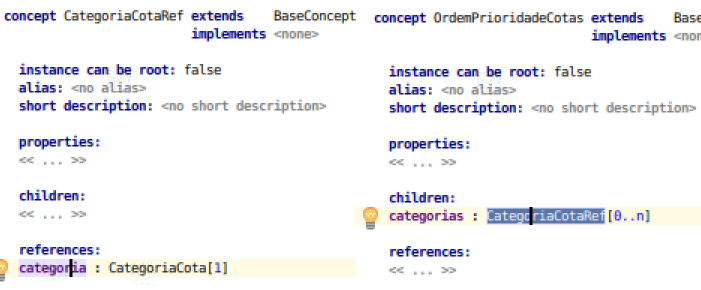
\includegraphics[width=\textwidth]{chapters/dslcotas/mps/imagens/references.png}}

\par\medskip\textbf{Fonte:} Elaborada pelo autor (2020). \par\medskip

\end{figure}



\newpage
Por fim, o conceito \texttt{Distribuicao} é o responsável por armazenar a árvore de distribuição, iniciando com a \texttt{CategoriaCota} raiz, na qual contém uma sigla, uma descrição, uma \texttt{Expression} onde será preenchida a reserva de vaga (percentuais fixos ou itens de \texttt{Configuracao} pré-definidos) e também uma lista de categorias filhas. 

Na Subseção \ref{sub:sec:editores}, serão apresentados os editores criados para definição da sintaxe de cada conceito definido na modelagem.


\subsection{\textit{Editores de conceitos}}
\label{sub:sec:editores}
O \gls{MPS} oferece aos projetistas uma abordagem de definição de sintaxe abstrata por meio de editores construídos com a notação de células. O \textit{designer} da linguagem combina as células do editor e as posiciona de maneira a refletir o layout final desejado da notação \cite{mpsCookBook}. 

Por padrão os elementos \texttt{Concepts} não possuem um editor associado, o editor padrão permite a edição direta da \gls{AST} pelo usuário da linguagem. No entanto, o editor padrão não é de simples entendimento para os usuários finais da linguagem, sendo necessário definir como aquele conceito deverá ser apresentado e editado pelo usuário.

Nesse sentido a Figura \ref{fig:editors}, apresenta a lista de editores criados para a DSL de cotas. As definições desses editores são apresentadas a seguir.

\begin{figure}[ht!]
\centering

\caption{\textmd{Editores de conceitos da DSL Cotas}}
\label{fig:editors}
\fcolorbox{gray}{white}{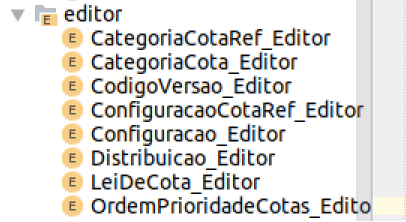
\includegraphics[width=0.85\textwidth]{chapters/dslcotas/mps/imagens/editors.png}}

\par\medskip\textbf{Fonte:} Elaboração do autor (2020) \par\medskip

\end{figure}




O primeiro editor \texttt{LeiDeCota\_Editor} é responsável pela organização das informações relevantes para o modelo de cotas, na Figura \ref{fig:editorleicota} observa-se que ele é composto por uma coleção de células organizadas verticalmente, essa coleção é representada por \texttt{'[-' e '-]'}. Dentro de cada linha da coleção é possível utilizar propriedades básicas do conceito, como por exemplo o campo \texttt{name}. 

\begin{figure}[ht!]
\centering

\caption{\textmd{Editor do conceito LeiDeCota}}
\label{fig:editorleicota}
\fcolorbox{gray}{white}{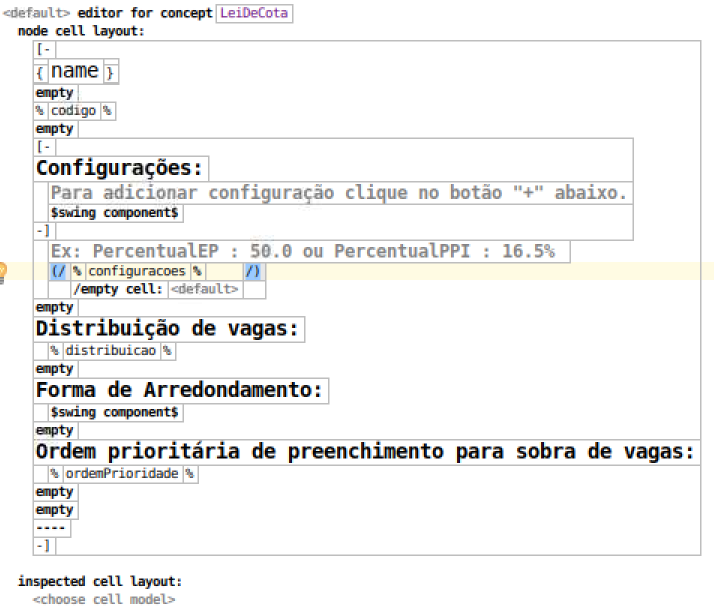
\includegraphics[width=0.85\textwidth]{chapters/dslcotas/mps/imagens/editorleicota.png}}

\par\medskip\textbf{Fonte:} Elaboração do autor (2020) \par\medskip

\end{figure}




\newpage
Também é permitido criar elementos estáticos para descrição de seções, como no caso do texto "Distribuição de Vagas" e referenciar os elementos \texttt{childrens} do conceito, por exemplo, \texttt{\%configuracoes\%}. No entanto, para que os elementos filhos sejam apresentados adequadamente para o usuário é necessário também definir o respectivo editor.

Por se tratar de um editor de múltiplas projeções, é possível inserir nos editores do \gls{MPS} alguns recursos gráficos disponíveis em sua linguagem base, Java, como por exemplo elementos de \texttt{JTable} e \texttt{JButton} das bibliotecas gráficas \texttt{swing}. A Figura \ref{fig:swingbutton} demonstra um exemplo de como a célula \texttt{\$swing\_component\$} é implementada para inserir o botão de adição de novas configurações na DSL.

\begin{figure}[ht!]
\centering

\caption{\textmd{Exemplo de componente de projeção gráfica}}
\label{fig:swingbutton}
\fcolorbox{gray}{white}{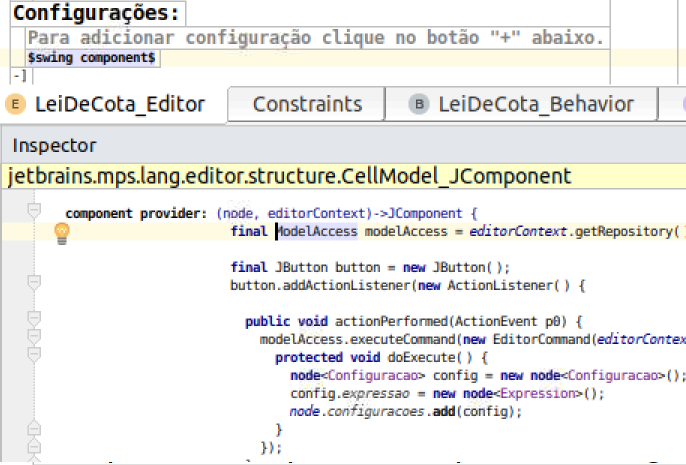
\includegraphics[width=0.75\textwidth]{chapters/dslcotas/mps/imagens/swingbutton.png}}

\par\medskip\textbf{Fonte:} Elaboração do autor (2020) \par\medskip

\end{figure}



Com objetivo de simplificar a edição da árvore de distribuição de vagas para o usuário final da DSL, foi utilizado o recurso \texttt{table} (\texttt{de.slisson.mps.tables}), que se trata de um plugin disponibilizado pelo pacote do \texttt{Mbeddr}\footnote{O Mbeddr é uma coleção de pacotes utilitários e extensões do MPS que permite a criação de muitos tipos diferentes de linguagens no \gls{MPS}.}. Segundo , as tabelas podem ser usadas para representar coleções de dados estruturados ou apresentar preocupações bidimensionais.

Nesse sentido, na Figura \ref{fig:tableeditor} é possível observar o \texttt{CategoriaCota\_Editor} onde as categorias filhas existentes são renderizadas com esse \textit{plugin} por meio dos comandos \texttt{table\{\}} e \texttt{getHeaders}, onde são iterados todos os seus filhos, de modo que as categorias sejam divididas por linhas indicando a sigla da categoria e o respectivo número de contagem de categorias, resultando no exemplo da Figura \ref{fig:tableeditorres}.

\begin{figure}[ht!]
\centering

\caption{\textmd{Editor com o plugin \texttt{table} do \texttt{Mbeddr}}}
\label{fig:tableeditor}
\fcolorbox{gray}{white}{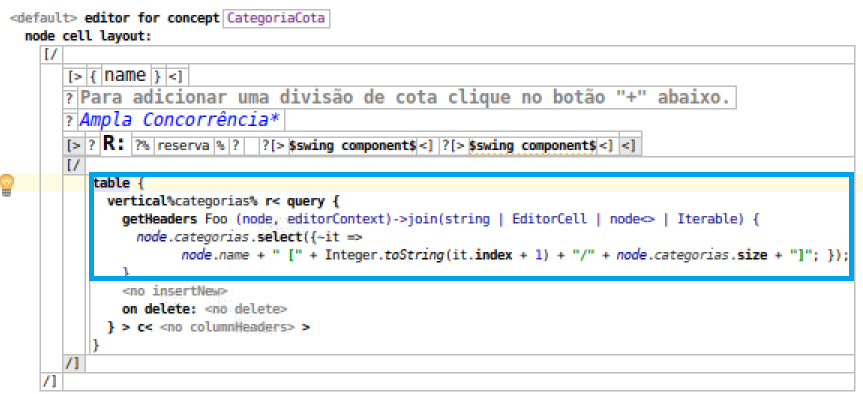
\includegraphics[width=0.95\textwidth]{chapters/dslcotas/mps/imagens/table.png}}

\par\medskip\textbf{Fonte:} Elaboração do autor (2020) \par\medskip

\end{figure}



\begin{figure}[ht!]
\centering

\caption{\textmd{Exemplo de resultado com uso do plugin \texttt{table}}}
\label{fig:tableeditorres}
\fcolorbox{gray}{white}{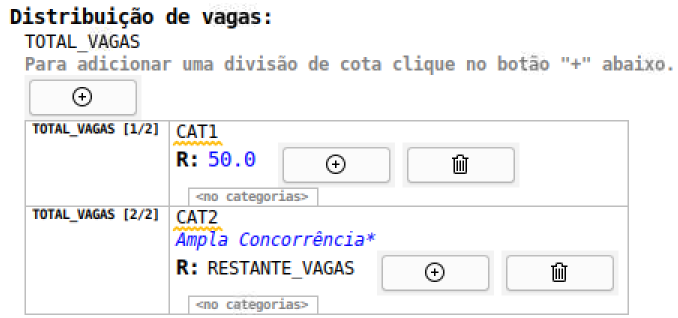
\includegraphics[width=0.95\textwidth]{chapters/dslcotas/mps/imagens/tableres.png}}

\par\medskip\textbf{Fonte:} Elaboração do autor (2020) \par\medskip

\end{figure}



\newpage
Após a definição de editores para todos os conceitos do modelo da linguagem, foi necessário utilizar o recurso de \texttt{constraints} para criar restrições de escopo para acesso às referências entre os elementos da linguagem. Esse detalhamento é observado na Seção \ref{sub:sec:constraints}.

\newpage
\subsection{\textit{Restrições de escopo}}
\label{sub:sec:constraints}

\subsection{\textit{Comportamento dos elementos de conceito}}
\label{sub:sec:comportamentos}

\subsection{\textit{Sistema de tipos}}
\label{sub:sec:typesystem}

\subsection{\textit{Gerador textGen}}
\label{sub:sec:texgen}